\section{Compiling data-plane algorithms}
\label{s:compiler}

\begin{figure}
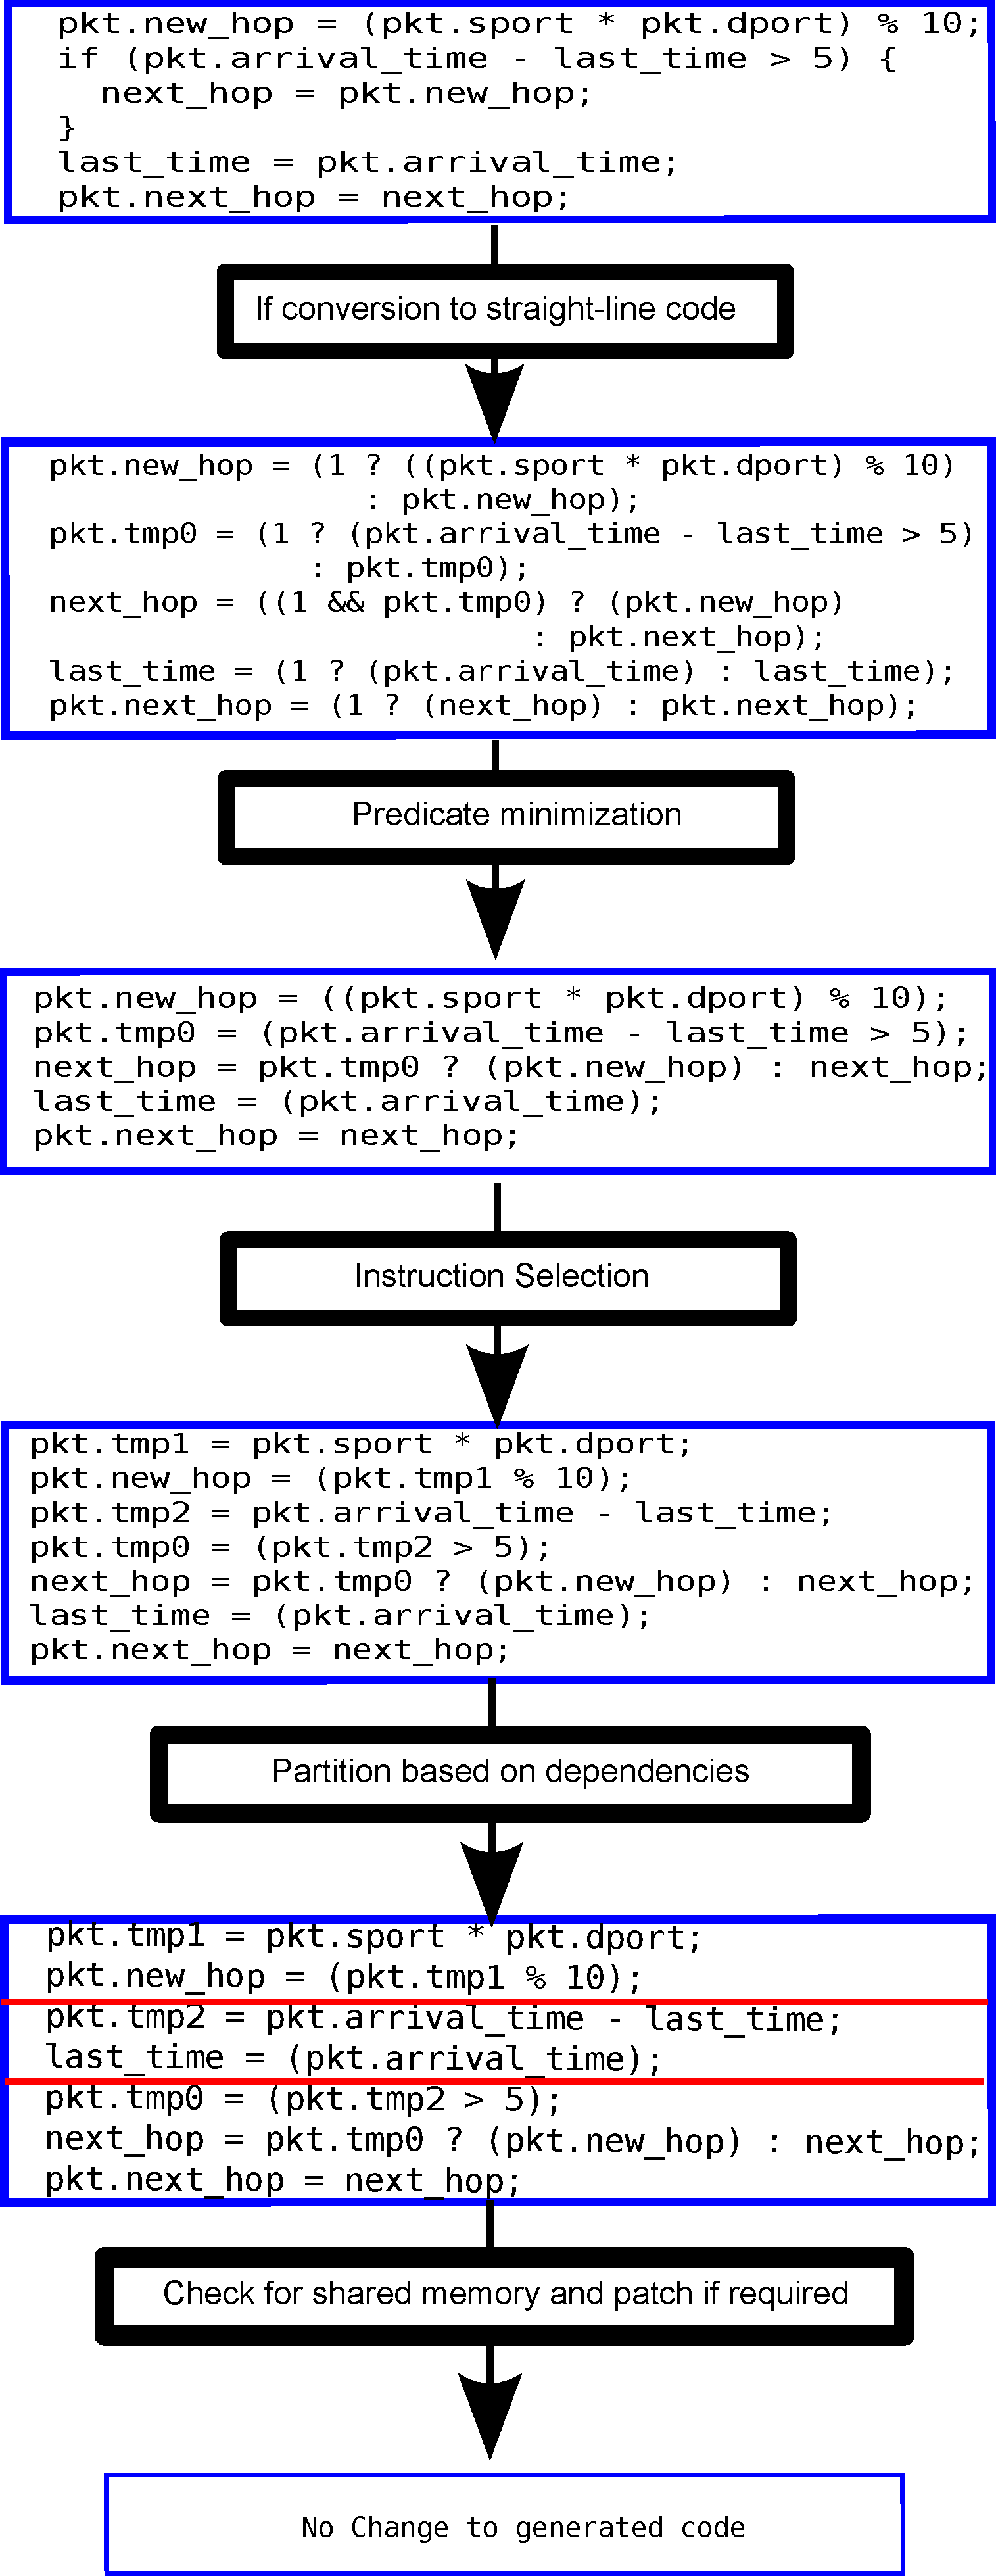
\includegraphics[width=\columnwidth]{compiler_flow.pdf}
\caption{The flow of code through the compiler}
\label{fig:flow}
\end{figure}

Our compiler takes code written in \pktlanguage and translates it into P4. This
source-to-source approach lets us focus on correctness issues when translating
\pktlanguage into P4 and lets a P4 compiler handle backend optimizations such
as table placement using target-specific information~\cite{lavanya_compiler}.
It also allows us to automatically leverage ongoing industry work on P4
compilation to hardware targets~\cite{netronome, xilinx}.

Figure~\ref{fig:flow} provides a high-level overview of the input and output to
the compiler for the running example that we use throughout this section: load
balancing using flowlet switching~\cite{flowlets}.  We structure the compiler
as a sequence of passes and describe each of them in turn below. 

%%TODO: Remember to get rid of this in the actual compiler
%%\subsection{Turning packet variables into local variables}

\subsection{Converting to straight-line code}
A general transaction body can contain convoluted control flow using if-else
statements. As an extreme example, consider the source code for CoDel:
\url{http://queue.acm.org/appendices/codel.html}. Control flow complicates
dependence analysis. We eliminate control flow by transforming if-else
statements using the ternary operator, starting from the innermost if
statements and recursing outwards using a well-known procedure called if
conversion~\cite{allen_if_conversion}.  This transformation creates
straight-line code, where control always passes from one statement to the next
without any branching.

\subsection{Predicate minimization}
Next, we simplify the predicates used in the ternary operator if possible.  In
the process, if we find the predicate is always true, we get rid of the ternary
operator altogether.

\subsection{Instruction selection}
We next replace portions of the straight-line code with equivalent code that
maps 1:1 to action primitives provided by the underlying hardware. While this
step does require knowledge of the action primitives supported by the
underlying hardware, P4 today already provides action primitives that map
1:1 to those provided by the underlying hardware, allowing us to carry out
instruction selection at the source level itself.
%Anirudh->Alvin: Ok, this is my interpretation of instruction selection
%TODO: Maybe we should just call it action primitive selection?

As a contrived example, if the underlying hardware supports read and write
operations on stateful memory, but does not support atomic increment operations
on stateful memory, we would have to replace the statement: \texttt{x = x + 1;}
with three statements:
\begin{verbatim}
int tmp1 = x;
int tmp2 = tmp1 + 1;
x = tmp2;
\end{verbatim}

Other examples of instruction selection include ``flattening''
expressions~\cite{expression_flattening} with deep ASTs into a canonical form
where the right hand side of each assignment is a simple expression that
doesn't contain any expressions within it. These simple expressions would then
map 1:1 to underlying hardware constructs.

\subsection{Partitioning based on dependencies}

% We need to mention how forward dependencies are ok: you can write a packet
% field to an updated value of the state variable.  You can also write a packet
% field to the previous value of the state variable.
%TODO: Get rid of semicolons in the partitioned output.

After instruction selection, the resulting straight-line code maps 1:1 to the
underlying hardware. At this stage, the code is correct if executed in a
straight-line assuming exactly one packet ever executes the code. A
straightforward partitioning simply assigns each instruction to a separate
stage, but is wasteful. Many instructions may have no dependencies between them
and can be executed in parallel.

To determine a better partitioning, we carry out the following sequence of steps:
\begin{enumerate}
\item If there are N instructions that read or write the same state variable,
we move the last $N-1$ of these to be as close to the first one as possible
while respecting Read-After-Write dependencies. This helps us avoid
recirculation unless absolutely necessary.
\item We assign each instruction to its own stage.
\item We then run an iterative algorithm that combines two adjacent stages if
there are no Read-After-Write or Write-After-Write dependencies between any
pair of instructions in each stage, stopping when no further stages can be
combined\footnote{Note that we don't need to consider Write-After-Read dependencies
between instructions because the underlying hardware executes parallel actions within
a stage simultaneously, which preserves the right semantics for Write-After-Read
depenendencies, whether between packet variables or state variables.}
\end{enumerate}

\subsection{Detecting memory sharing across stages}
In our entire discussion so far, we make no distinction between stateful
variables and packet-local variables. This is because, if there is only a
single packet in the system, there is no distinction between the two.

In this pass, we scan the partitioning looking for stateful variables (any
globally declared variable), and checking if any stateful variable is read in
one stage and then written in a subsequent stage. If this is the case, that
stateful variable needs to be shared across stages and the best we can do is to
approximately emulate such sharing using recirculation.

Instead, if a stateful variable is written in exactly one stage, but read in
multiple stages following the stage that it is written in, we can achieve this
effect by simply writing the stateful variable into a packet field that then
carries the value to subsequent stages.

We note here that this pass relies on the instruction selection pass to
determine a good set of instructions that map closely to the hardware. For
instance, if instruction selection cannot rewrite the set of sequential
statements: \texttt{x = x + y; y = y + x;} into the tupled form \texttt{(x, y)
= (x + y, 2 * y + x);}, then the one-packet compiler will move \texttt{y = y +
x;} into the stage following \texttt{x = x + y;} causing spurious memory
sharing.

\subsection{Patching code to achieve memory sharing}
The previous pass might detemine that a stateful variable needs to be shared
across stages, because it is read in one and written in a stage downstream. If
this is the case, we need to clone a packet and recirculate back to the first
stage of the pipeline that it needs to be read in.

Because the pipeline needs to keep up with line rate and cannot be paused, we
the implementation needs to handle both new data packets and recirculated
cloned packets that carry state updates. We achieve this by patching the code
created by the previous pass to execute the algorithm on batches of packets
instead rather than every packet. We outline the patching procedure below.

The first stage maintains a state variable $in\_progress$ to denote whether the
algorithm is currently being executed or not. When the first data packet is
received, it set $in\_progress$ to true, executes whatever other operations
need to be executed as part of the algorithm itself, and passes the packet
downstream to other stages with an $execute\_algorithm$ field set in the
packet. The remaining stages simply follow the lead of the first stage and
execute the algorithm if the $execute\_algorithm$ field is set, accumulating
writes to shared variables in packet fields. At the end of the last stage, we
clone a packet containing all these writes and recirculate it back into the
pipeline to update all state variables. Once all state is updated, we
recirculate the cloned packet a second time to reset the $in\_progress$ bit to
false again.

We are still left with the question of what to do when $in\_progress$ is true
and a new data packet is received in the pipeline. For now, we simply pass
these packets through unchanged, although there are likely other alternatives.
This pass-through mode corresponds roughly to transactional semantics on
batches of packets, where the batch size is the number of packets that arrive
during the time it takes to recirculate a packet twice. While this may not be a
reasonable solution for all data-plane algorithms, some meausrement algorithms
can work on a sampled stream of packets with graceful performance degradation.
We evaluate this performance degradation quantitatively in
\S\ref{ss:evaluation_approx}, leaving a more accurate characterization of possible
approximations to future work.

\subsection{Translating to P4}
As a final step, we translate the partitioned code (patched, if required)
into P4. This is a conceptually straightforward process:
\begin{enumerate}
\item We add newly created temporary variables to the header and parser
specifications so that P4 can automatically generate the parser state machine.
\item We create a P4 logical table for each partition.
\item The set of packets on which the algorithm will run is specified using
an appropriate match type (exact, ternary, or longest-prefix) on specific
header fields within each logical table.
\item We create a P4 action in each logical table from the code in the
corresponding partition.
\item Lastly, the control-flow between P4 tables mirrors the order of
partitions.
\end{enumerate}

%Advanced idioms:
%--> Pipeline wide memory using recirculation primitive.
%--> Tupled Stateful operations: <x, y> <--- f(x, y).
%--> Multiply accumulate (MAC).
%
